\section{Studio di fattibilità}

\subsection{Contesto d'uso}
Dalle analisi precedenti di user research e valutazione di sistemi
esistenti si può fare un quadro del contesto d'uso dell'applicazione
proposta.
Vedremo in particolare qual'è il target d'utenza, quali sono i task da
prendere in considerazione e quali sono i possibili vincoli tecnici e
ambientali.

\subsubsection{Target d'utenza}
Come emerge dalla user research il target d'utenza previsto è molto
eterogeneo, infatti non si sono riscontrati dei restrittivi limiti di
età, istruzione o competenze culinarie.\\
Forse l'unica vera restrizione riguarda la nazionalità degli utenti
in quanto si è deciso di concentrare
l'attenzione verso l'utenza italiana. Questa scelta è nata dall'analisi
delle statistiche le quali suggeriscono che l'Italia è una delle
prime nazioni nel mondo per quanto riguarda la passione culinaria
\ref{fig:cooking-country}. A conoscenza di ciò, focalizzarsi su un
utenza internazionale avrebbe potuto confondere gli italiani, poco familiari
con lo stile culinario non tradizionale. Ad esempio la colazione
italiana prevede un pasto molto rapido a differenza di molte colazioni
estere e la suddivisione delle portate in ``primo'' e ``secondo'', le quali
identificano già la categoria della pietanza, non è molto comune
all'estero.

\subsubsection{Task}
A seguito delle valutazioni dei sistemi esistenti, è risultato opportuno
rivisitare la lista dei task già definita nello user research
\ref{tasks}, con
l'idea di far forza sul contesto nel quale le applicazioni esistenti
mostrano le loro debolezze.

\begin{enumerate}
\label{tasks}

\item Impostare il livello di preparazione culinaria
\item Accedere alla documentazione/help dell'applicazione

\item Ricerca di una ricetta per nome.
\item Ricerca di una ricetta per ingredienti.

\item Ricerca di una ricetta sfogliando le categorie.

\item Filtro di una ricerca in base agli ingredienti.
\item Filtro di una ricerca in base alle intolleranze/allergie/diete.

\item Individuare la difficoltà di preparazione e il costo di una ricetta.
\item Individuare gli ingredienti necessari alla preparazione di una ricetta.
\item Distinguere le varie fasi di una preparazione della ricetta.
\item Distinguere la vista passo-passo della preparazione dalla visione complessiva della ricetta.
\item Visionare un video di presentazione della ricetta
\item Condividere una ricetta sui social network.
\item Creare un menù completo selezionando una lista di ricette.
\item Aggiungere/Rimuovere una ricetta al menù già creato.
\item Cercare un menù consigliato da CookApp.

\item Inserire una nuova ricetta nel database dell'applicazione.
\item Interagire con la community rispondendo a problemi degli utenti.
\item Chiedere consiglio alla community creando un nuovo topic.
\item Chiedere aiuto "live" alla community riguardo un particolare passaggio della ricetta oppure riguardo agli ingredienti

\item Salvare/Rimuovere una ricetta nei preferiti.
\item Salvare/Rimuovere un menù nei preferiti.

\item Accedere alla lista della spesa.
\item Inserire/Rimuovere gli ingredienti di una ricetta nella lista della spesa.
\item Inserire/Rimuovere gli ingredienti di un menù nella lista della spesa.

\item Votare e commentare le ricette ed i menu.

\item Visualizzare il progresso della preparazione del menù e della singola ricetta



\item Trova i punti vendita degli ingredienti della lista della spesa.
\item Interagire con la mappa del percorso mediante lo smartwatch per strada e nel punto vendita.
\item Identificare il prodotto acquistato con l'NFC dello smartwatch eliminando la relativa voce dalla lista della spesa.
\item Aggiungere/confermare una voce nella lista della spesa con lo smartwatch.


\item Avanzare con le fasi di preparazione passo-passo mediante messaggi vocali.
\item Text-to-Speech delle fasi di preparazione di una ricetta.


\end{enumerate}

Vedremo in seguito gli approcci delle applicazioni già esistenti verso
questi task e le funzionalità da progettare nella nostra applicazione
affinché tali task possano essere eseguiti al meglio.


\subsubsection{Vincoli tecnici ed ambientali}
L'applicazione è pensata per essere utilizzata in ambienti probabilmente
molto caotici, in cui l'attenzione dell'utente potrebbe essere
facilmente catturata da altri elementi del contesto. Questo aspetto è
stato riscontrato anche durante le osservazioni del contextual inquiry:
i tre studenti si sono facilmente distratti a causa dell'euforia della
novità, mentre la signora Antonietta si è fatta distrarre dalla
discussione con la sorella. A rafforzare tale supposizione sono i
risultati del sondaggio i quali mostrano che il livello di esperienza
culinaria media è medio-bassa.
Un vincolo per l'appliczione
potrebbe essere infatti la disposizione disordinata degli ingredienti
e degli atrezzi nella cucina, che potrebbe impediere un comodo
raggiungimento e utilizzo del
device, scoraggiando l'utente all'approccio tecnologico. Inoltre
avere le mani impegnate potrebbere rendere l'applicazione inutilizzabile
in alcuni casi, soprattuto se l'ausilio dei comandi vocali non fosse
previsto. Ad ogni modo anche nche nel caso in cui fossero previsto comandi vocali,
un ambiente molto caotico potrebbe essere un vincolo.\\
Il tutto suggerisce di progettare un applicazione la cui interfaccia sia
molto semplice, immediata e che riduca il carico di stress
percepito dall'utente.

\subsection{Personas}
\begin{table}[H]
	\begin{centering}
	\begin{tabular} { | r  p{10cm} | }
		\hline
		\multirow{2}{*}{
			\begin{minipage}{.18 \textheight}
				\vspace{0.1in}
				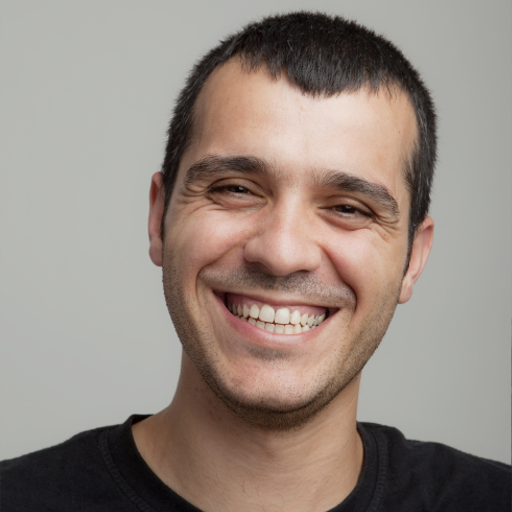
\includegraphics[width=\linewidth]{img/personas/filippo.png}
			\end{minipage}
		}
		 & \vspace{0.1 in}\Large\textbf{Filippo} \\ 
		& \vspace{0.1 in}\large{\emph{``Anche se viaggio molto per catturare il mondo,
cucinare all'estero mi fa
		sentire sempre a casa. Sempre pronto a re-inventare la tradizione anche con
		ingredienti difficili.''}}\\[8ex] 
		\hline
		\textbf{Anni} & 36 \\ \hline
		\textbf{Occupazione} & Fotografo \\ \hline
		\textbf{Famiglia} & {Nonostante i frequenti viaggi, ha uno
studio e un domicilio a Rimini, città in cui è cresciuto con la sua
famiglia. Ogni circa due settimane Filippo fa visita ai genitori per il
pranzo domenicale insieme alla sua ragazza spagnola con cui convive.} \\
\hline
		\textbf{Profilo Tecnico} & Dopo il liceo artistico ha vissuto 5
anni in Spagna, lavorando sia come cameriere in un ristorante italiano
sia come impiegato in un'agenzia di viaggi. Tornato in italia ha poi
deciso di seguire la sua passione per la fotografia iscrivendosi
all'accademia delle belle arti. Terminati gli studi ha iniziato a
viaggiare in tutto il mondo pubblicando le sue foto in un blog wordpress gestito
da lui stesso. Da 2 anni ha aperto un proprio studio fotografico in
Italia. \\ \hline
		\textbf{Hobby} & Ha sempre avuto una grande passione per il
rugby, sport che ha abbandonato dopo l'università anche se continua a
seguirlo assiduamente. \\ \hline
		\textbf{Rapporto con la cucina} & Nonostante gli piaccia molto
la cucina spagnola e quella asiatica, rimane molto legato alla cucina
tradizionale italiana. Cucina spesso e volentieri piatti italiani molto
semplici ma che comunque sono molto graditi dalla sua ragazza spagnola.
\\ \hline
		\textbf{Rapporto con la tecnologia} & Prima di quest'anno non
aveva mai considerato
l'acquisto di un tablet, essendo abituato a lavorare sempre il laptop 
per necessità di utilizzo di software di editing
d'immagini. Dopo avero provato un tablet surface, che permette di
passare in modalità desktop agganciando una tastiera al dispositivo, ha
deciso di comprarne uno, affascinato dalla possibilità di poter
continuare ad utilizzare i suoi software con interfaccia destkop e
sfruttare allo stesso tempo l'estrema mobilità e le app di un tablet.
Ha anche una buona familiarità con il Web avendo gestito in passato un proprio
blog di foto ed una pagina facebook. Lo scorso natale la ragazza gli ha
regalato uno smartwatch che inizialmente non trovava di particolare
utilità, ma dopo aver visto che gli permette di visualizzare a distanza
la ripresa della fotocamera del suo smartphone ha iniziato ad
utilizzarlo regolarmente come supporto alla fotografia. Infatti ha
intenzione di acquistare prossimamente una nuova reflex con sistema
operativo Android da integrare al suo smartwatch.
\\ \hline
	\end{tabular}
	\end{centering}
\end{table}


\begin{table}[H]
	\begin{centering}
	\begin{tabular} { | r  p{10cm} | }
		\hline
		\multirow{2}{*}{
			\begin{minipage}{.18 \textheight}
				\vspace{0.1in}
				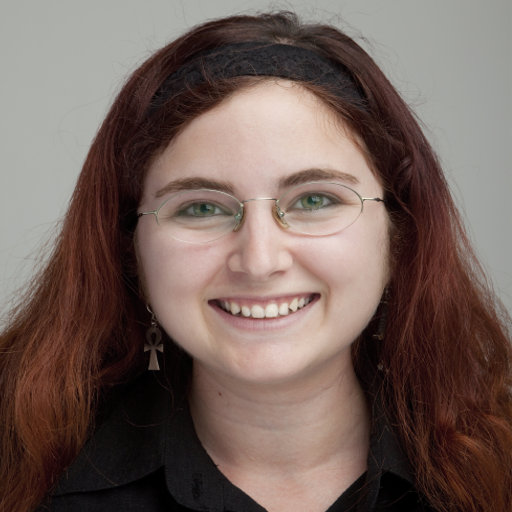
\includegraphics[width=\linewidth]{img/personas/flora.png}
			\end{minipage}
		}
		 & \vspace{0.1 in}\Large\textbf{Flora} \\ 
		& \vspace{0.1 in}\large{\emph{``I love dogs as much as I
love Italian guys. They are all handsome and funny and I am trying to
	lose some weight to look prettier. Maybe some of them will notice
me.''}}\\[8ex] 
		\hline
		\textbf{Anni} & 28 \\ \hline
		\textbf{Occupazione} & Dottoranda in geologia \\ \hline
		\textbf{Famiglia} & {Ha vissuto a Glasgow in Scozia con la madre
ed il fratello maggiore fino ai tempi del liceo. Si è poi trasferita in
un campus ad
Edimburgo per frequentare l'università. Data la breve distanza tra le
due città non ha sofferto il distacco dalla famiglia tornando a casa
quasi ogni fine-settimana. Da due anni ha lasciato la Scozia e le manca molto il
fratello con cui ha un rapporto molto speciale maturato dopo il
divorzio dei genitori.} \\
\hline
		\textbf{Profilo Tecnico} & Si è specializzata in geologia presso
l'università di Edimburgo. Ha ottenuto poi una borsa di studio per un
dottorato di ricerca all'Università di Bologna. Non ha mai lavorato al
di fuori dell'ambito accademico.\\ \hline
		\textbf{Hobby} & Ama i cani e prendersi cura di loro. Nel
fine-settimana lavora occasionalmente come dog-sitter, non molto per
bisogni economici ma per passare un po' di tempo con i cani visto che ha
dovuto lasciare il suo terrier in Scozia. \\\hline
		\textbf{Rapporto con la cucina} & Come tutti gli scozzesi ama
la cucina italiana, in particolare il gelato e la lasagna. Nei
primi mesi di dottorando in Italia ha messo su qualche chilo e ha deciso
quindi di iniziare una dieta. Spesso però, soprattuto nei periodi dalle
scadenze accademiche, non riesce a resistere ad una buona pizza o alla
trattoria bolognese,
sia per dare sfogo allo stress, sia per l'impegno di fare spesa e
cucinare.\\ \hline
		\textbf{Rapporto con la tecnologia} & Utilizza quotidianamente
il PC per fare ricerca e lo smartphone per messaggiare con gli amici.
Quando è a casa predilige il tablet perchè spesso effettua lunghe
videochiamate con la madre con cui comunica anche durante lo svolgimento
di altre mansioni, spostandosi da una stanza all'altra.\\ \hline
		\textbf{Altri particolari} & Condivide un appartamento con altri
due studenti molto più piccoli di lei. Periodicamente organizzano feste
in casa anche infrasettimanalmente. Lei ormai stanca delle feste
universitarie che si prolungano fino a tarda notte, si fa spesso ospitare
dall'amica Francesca in queste occassioni. Anche se prova una sorta di disagio per il
disturbo creato all'amica, ritiene sia l'unico modo per affrontare la giornata
succesiva.\\ \hline
	\end{tabular}
	\end{centering}
\end{table}

\begin{table}[H]
	\begin{centering}
	\begin{tabular} { | r  p{10cm} | }
		\hline
		\multirow{2}{*}{
			\begin{minipage}{.18 \textheight}
				\vspace{0.1in}
				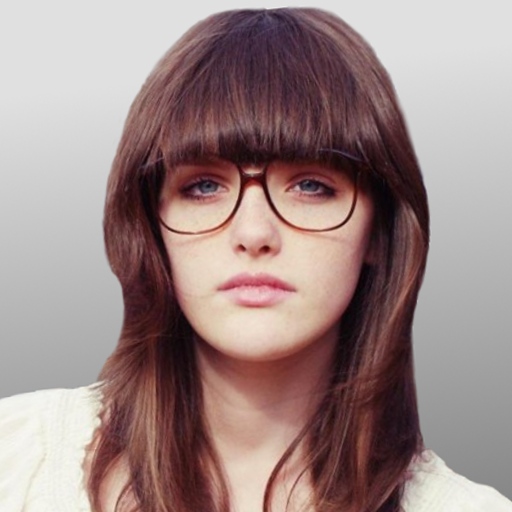
\includegraphics[width=\linewidth]{img/personas/francesca.png}
			\end{minipage}
		}
	 	& \vspace{0.1 in}\Large\textbf{Francesca} \\ 
		& \vspace{0.1 in}\large{\emph{``Ho una gran passione per l'indie rock e
il vintage design. Da due anni ho deciso di diventare vegetariana, sia
per rispettare la mia salute sia per contrastare lo sfruttamento animale
delle multinazionali.''}}\\[8ex] 
		\hline
		\textbf{Anni} & 27 \\ \hline
		\textbf{Occupazione} & Giornalista tirocinante \\ \hline
		\textbf{Famiglia} & È figlia unica ed è stata cresciuta 
a Verona dai genitori, che le hanno permesso sempre di inseguire le sue
passioni.\\ \hline
		\textbf{Profilo Tecnico} & Dopo aver terminato il liceo classico
di Verona, si è trasferita a Bologna per frequentare l'università.
Laureata da un anno in lettere e filosofia ha iniziato da qualche mese
un tirocinio retribuito in una nota testata giornalistica a Bologna. \\\hline
		\textbf{Hobby} & Nel tempo libero le piace cucire sciarpe e
capelli per lei e per il suo ragazzo. Il finesettimana non perde mai un
concerto indie rock e frequenta spesso i negozi dell'usato per alla
ricerca di oggettistica vintage. \\ \hline
		\textbf{Rapporto con la cucina} & È diventata vegeteriana dopo
aver lasciato Verona. Il suo cambio di alimentazione non è stato
drastico in quanto non le è mai piaciuta molto la carne. Il problema le
si presenta quando mangia fuori casa con altre persone, occasioni in cui
prestare attenzione agli ingredienti delle pietanze che mangia. \\ \hline
		\textbf{Rapporto con la tecnologia} & Si è sempre definita
riluttante alla tecnologia, prediligendo canali d'informazione più
classici rispetto al web. Ha utilizzato il PC per lunghi periodi
solamente per scrivere le sue tesi universitarie. Non possiede uno
smartphone e continua ancora ad utilizzare gli SMS.\\ \hline
		\textbf{Altri particolari} & Frequenta da pochi mesi un ragazzo
amante di cucina tipica emiliana. Nonostante i loro tipi di
alimentazione molto diversi, il cibo non è mai una causa di discussione. \\\hline
	\end{tabular}
	\end{centering}
\end{table}

\begin{table}[H]
	\begin{centering}
	\begin{tabular} { | r  p{10cm} | }
		\hline
		\multirow{2}{*}{
			\begin{minipage}{.18 \textheight}
				\vspace{0.1in}
				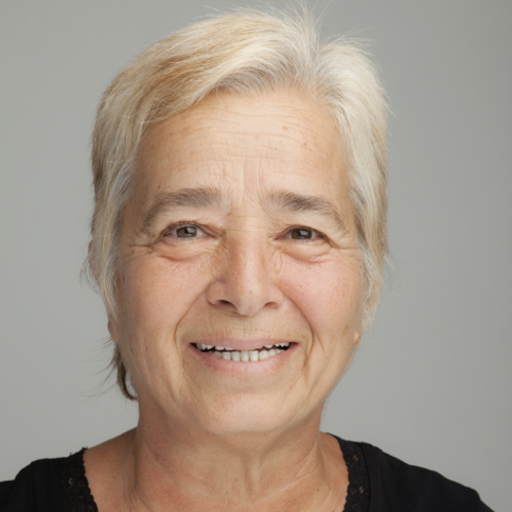
\includegraphics[width=\linewidth]{img/personas/maria.png}
			\end{minipage}
		}
	 	& \vspace{0.1 in}\Large\textbf{Maria} \\ 
		& \vspace{0.1 in}\large{\emph{``I miei figli vivono tutti in
città, ma io la montagna proprio non la lascio. Qui l'aria è buona e si
mangia bene, altro che i faste fud dove vanno i miei nipoti. Almeno con
il nuovo tablet che mi hanno regalato li vedo spesso con l'internet.''}}\\[8ex] 
		\hline
		\textbf{Anni} & 63 \\ \hline
		\textbf{Occupazione} & Pensionata \\ \hline
		\textbf{Famiglia} & Ha due figli maschi ed una femmina. I due
maschi vivono entrambi a Milano mentre la figlia vive a Napoli dopo
essersi sposata con un carabiniere conosciuto durante un suo periodo di servizio a
Milano. Quasi una volta al mese i figli di Milano vanno a trovarla a
Cusio, un piccolo paesino di montagna in provincia di Bergamo dove
tutt'ora vive. La signora Maria però, soffre molto la distanza con
l'altra figlia che riesce a vedere solo una volta l'anno durante le
feste natalizie. \\ \hline
		\textbf{Profilo Tecnico} & Ha lavorato per tutta la vita come
postina a Cusio e nei dintorni. Adesso si gode una meritata pensione. \\ \hline
		\textbf{Hobby} & Ha sempre avuto la passione per il ballo, che
coltiva con suo marito frequentando occasionalmente la balera del paese.
Oltre al liscio ha una vera ossessione per le telenovelas e tutti i
programmi TV condotti da Maria De Filippi.  \\\hline
		\textbf{Rapporto con la cucina} & A detta dei nipotini, abituati
alla cucina di città, la nonna Maria è la cuoca
più brava del mondo. Abituata ad una cucina molto tradizionale e
montana, il suo piatto forte sono i fagottini con funghi porcini e
Bitto, un formaggio di mucca tipico della Lombardia. Purtroppo il
marito della figlia che vive a Napoli è intollerante al lattosio e
quando c'è anche lui a tavola questo piatto diventa un tabù.\\ \hline
		\textbf{Rapporto con la tecnologia} & Non ha mai utilizzato un
computer. Per molto tempo i figli milanesi hanno cercato di farle
utilizzare uno
smartphone ma con scarso successo in quanto Maria, a causa
dell'abbassamento della vista, ha riscontrato che si stanca molto
	durante l'interazione con i piccoli schermi degli smartphone. I
figli hanno deciso quindi di regalarle un tablet in quanto ha uno schermo più
grande rispetto agli smartphone e molte applicazioni pensate appositamente per gli anziani.
Alla signora Maria sembra piaciere il nuovo dispositivo e, nonostante abbia dei 
tempi molto lenti di apprendimento, è molto motivata ad
imparare come utilizzarlo in quanto le permette di
videochiamare la figlia che vive a Napoli e vedere le foto dei nipotini
mentre crescono. \\ \hline
		\textbf{Altri particolari} & Il marito della signora Maria è
molto orgoglioso delle sue origini nordiche e non ha mai preso in
simpatia il carabiniere napoletano che la figlia ha sposato. \\\hline

	\end{tabular}
	\end{centering}
\end{table}

\begin{table}[H]
	\begin{centering}
	\begin{tabular} { | r  p{10cm} | }
		\hline
		\multirow{2}{*}{
			\begin{minipage}{.18 \textheight}
				\vspace{0.1in}
				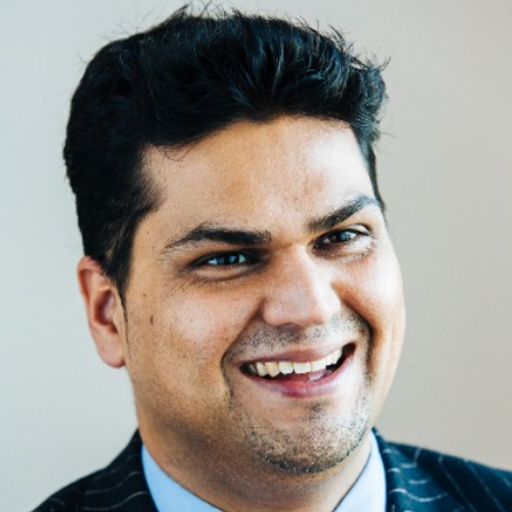
\includegraphics[width=\linewidth]{img/personas/giuseppe.png}
			\end{minipage}
		}
	 	& \vspace{0.1 in}\Large\textbf{Giuseppe} \\ 
		& \vspace{0.1 in}\large{\emph{``I milanesi parlano tutti male di
Napoli, ma dopo esserci stati non se ne vogliono più andare. Mia moglie
milanese infatti adesso ama la mia città tanto quanto ama me. Solo noi abbiamo il
sole, il mare, la pizza e il babà.''}}\\[8ex]
		\hline
		\textbf{Anni} & 42 \\ \hline
		\textbf{Occupazione} & Maresciallo dei Carabinieri \\ \hline
		\textbf{Famiglia} & Ha sposato Chiara, una donna del nord
Italia, conosciuta durante un periodo di servizio a Milano. Hanno una
bambina di 6 anni.\\ \hline
		\textbf{Profilo Tecnico} & Dopo le scuole superiori si
arruola all'Accademia Militare per intraprendere gli studi in
Giurisprudenza e diventare un ufficiale. Viene in seguito reclutato come
maresciallo dell'Arma dei Carabinieri. Attualmente è in comando stabile
presso una caserma della periferia di Napoli. \\\hline
		\textbf{Hobby} & Fuori servizio, quando non passa del tempo con
la sua famiglia, pratica il tiro con l'arco.\\ \hline
		\textbf{Rapporto con la cucina} & È di buona forchetta e gli
piace molto cucinare. Ha una buona esperienza con i fornelli maturata
durante il periodo dell'Accademia Militare e ama i piatti tipici
Napoletani e gli ingredienti del sud Italia. Negli ultimi anni però il
medico gli ha proibito di consumare latticini a causa di un intolleranza al
lattosio. Giuseppe ha impiegato diverso tempo per accettare la sua
intolleranza avendo avuto sempre un debole per la mozzarella di bufala.\\ \hline
		\textbf{Rapporto con la tecnologia} & Utilizza il PC in caserma
esclusivamente tramite il sistema software dei Carabinieri per risolvere
le pratiche quotidiane. A casa utilizza sporadicamente il
laptop della moglie giusto per navigare e riprodurre video. Possiede uno
smartphone ma lo utilizza principalmente per le classiche telefonate e fotografare i
piatti ai ristoranti.\\ \hline
	\end{tabular}
	\end{centering}
\end{table}
\subsection{Scenari d'uso}
\begin{enumerate}

\item Filippo nell'ultimo viaggio in brasile ha conosciuto Paulo, un
impiegato in banca appassionato di fotografia. Filippo ospiterà per un
weekend Paulo
e suoi 3 amici che stanno visitando l'Italia. A tal proposito voleva
preparare una cena tipica italiana di benvuto. Per non risultare banale,
si affida a
CookApp scegliendo uno tra i menù preimpostati consigliatii. Il menù
scelto prevede per antipasto ``Capasanta atlantica con gatzpacho fresco
e croccante di pane'', per primo dei ``Ravioletti ripieni di cacio e
pepe'' e per secondo una ``tagliata di fassona piemontese''. Decide però
di sostituire il secondo con ``Spiedini di gamberi'', un piatto scelto tra i ``Tipici della
zona''. Infine come dolce, inserisce un classico ``Tiramisù'' nel menù.
Dopo aver ultimato le modifiche al menù aggiunge tutti gli ingredienti
necessari alla lista della spesa. Dalla schermata della lista della
spesa Filippo cerca i punti vendita dove per poter acquistare gli
ingredienti e scegli quelli più vicino a casa. A questo punto esce di
casa seguendo il percorso verso i punti vendita selezionati,
visualizzati sulla mappa del suo smartwatch. Arrivato al primo punto
vendita lo smartwatch indica, tramite una mappa più dettagliata, le posizioni degli ingredienti delle
relative corsie del supermercato. Grazie al modulo NFC dello smartwatch,
Filippo scansiona il tag NFC dei prodotti da acquistare che vengono
automaticamente confermati sulla lista della spesa. Infine si dirige
alla cassa e effettua il pagamento di tutta la spesa posizionando lo
smartwatch al sensore della cassiera. 
Finita la spesa nei diversi punti vendita, Filippo torna a casa e
prepara una deliziosa cenetta per i suoi amici brasiliani.


\item Per le vacanze di Pasqua i coinquilini di Flora tornano a casa dalla famiglia, e
lei decide quindi di invitare per pranzo l'amica Francesca e il suo
ragazzo Enrico, per voler ricambiare la grande ospitalità che lei spesso
le offre. Flora vorrebbe realizzare un menù tipico Pasquale ma
solitamente era sempre tornata in Scozia per le vacanze e non ha idea di
cosa mangino gli italiani in queste occasioni.

Tramite l'applicazione
cookApp, già impostata in lingua inglese grazie al riconoscimento della lingua
di sistema del suo tablet, Flora accede alla categoria ``Holidays'' e alla
sottocategoria ``Easter'' trovando facilmente i piatti tipici pasquali. 
Si ricorda però che la sua amica Francesca è vegetariana quindi
seleziona il filtro di vista ``With vegetarian version'' che le permette
di visualizzare tutte le ricette che abbiano anche le istruzioni per
prepararne una variante vegetariana. Ha preferito questo filtro rispetto
a ``Vegetarian'' in quanto il ragazzo di Francesca è amante della carne e
così ha modo di prepare gli stessi piatti per tutti, ma in due versioni
diverse. Una volta individuate le ricette decide di aggiungerle ad un
nuovo menù personalizzato. CookApp inoltre, durante la consultazione
della categoria pasqua, suggerisce a Flora di decorare la
tavola con degli ovetti di pasqua, che all'apparenza sembrano delle
classiche uova sode decorative ma che poi riveleranno una simpatica sorpresa al
loro interno. Grazie a CookApp Flora riesce a preperare senza difficoltà
il pranzo pasquale a fare felici i suoi amici.


\item La signora Maria, in occasione della visita che le faranno
l'indomani i suoi figli da Milano, decide di preparare i fagottini al
Bitto che tanto piacciono al suo nipotino Marco. La mattina dopo Chiara, la
figlia di Maria che vive a Napoli, avverte sua madre che è in viaggio,
insieme a suo marito carabiniere Giuseppe e la loro bambina,
per andare a trovarla. Le dice anche che arriverrano per l'ora di pranzo, scusandosi
per non averglielo detto prima ma si sono
riusciti ad organizzare solamente all'ultimo momento. Maria è molto
felice che si riunirà tutta la famiglia anche se è un po' dispiaciuta
perchè non può più prepare i fagottini al Bitto inquanto Giuseppe è
intollerante al lattosio. Inoltre la decisione di Maria
altera l'animo del marito il quale sostiene che il carabiniere non è
davvero intollerante ma ha problemi con le mozzarelle napoletane perchè
contaminate dai rifiuti del sottosuolo campano. Non volendo far
dispiacere nessuno, la signora Maria prova a cercare su CookApp una
variante dei fagottini al Bitto per intolleranti al lattosio. In
particolare scrive ``fagottini al bitto'' nella barra di ricerca
selezionando il filtro ``Senza lattosio''. Non ottiene nessun risultato
ma CoockApp le chede se vuole rivolgersi alla comunità online per un
aiuto sulla ricetta ``Fagottini al bitto''. Maria pigia l'apposito
pulsante di conferma e tramite la casella di inserimento e il pulsante
di invio, pubblica la sua richiesta per la community. Ottiene nel giro
di qualche minuto una risposta di una ragazza di Sondrio che le
consiglia di utilizzare un composto di maionese e tofu. Maria seleziona
quest'ultimo ingrediente e ne compare una descrizione, oltre ad un
pulsante ``Dove comprare''. Maria lo pigia e compare una mappa di
supermercati nelle vicinanze. Nota che il supermercato più vicino che
hanno il tofu è a Bergamo, quindi chiede al figlio di Milano se può
passare a comprare questo ingrediente al supermercato di Bergamo. Infine
Maria prepara degli ottimi fagottini al tofu e maionese che non deludono
nessuno, neanche il marito, che nonostante aver riconosciuto la
differenza ammette che gli sono piaciuti.

\end{enumerate}
